\documentclass[a4paper, 11pt]{report}
\setcounter{tocdepth}{3}
\usepackage[utf8]{inputenc}
\usepackage[french]{babel}
\usepackage[T1]{fontenc}
\usepackage{graphicx}
\usepackage{xcolor}
\usepackage{booktabs}
\usepackage{tabularx}
\usepackage{fourier} 
\usepackage{array}
\usepackage{makecell}
\usepackage[top=2.5cm,bottom=2.5cm,right=2.5cm,left=2.5cm]{geometry}
\usepackage{amsmath}
\usepackage{xcolor}
\usepackage{colortbl,hhline}
\usepackage{subfig}
\usepackage{multirow}
\usepackage{comment}
\usepackage{makecell}

\usepackage{algorithmic,algorithm}

\renewcommand{\listalgorithmname}{Liste des \ALG@name s}

\definecolor{yacine}{RGB}{241,241,241}
\usepackage{tikz}
\def\checkmark{\tikz\fill[scale=0.4](0,.35) -- (.25,0) -- (1,.7) -- (.25,.15) -- cycle;} 

\usepackage[backend=bibtex,style=numeric,sorting=nty]{biblatex}
\nocite{*} %Ausgabe aller Bibliographieeinträges
\usepackage{hyperref}
\hypersetup{
    linktoc=all,     %set to all if you want both sections and subsections linked
}




\begin{document}
 
\begin{center}
\begin{tabular}{|c|}
\hline
Compte rendu de la présentation\\du 19\//03\//2018\textsl{•}\\
\hline

\end{tabular}
\end{center}


En présence de :\\
\begin{itemize}
\item Monsieur Mohand-Saïd HACID
\item Monsieur Emmanuel COQUERY
\end{itemize}


Déroulement de la séance :\\
Durant cette séance, j'ai d'abord commencé par présenter l'actuel avancement de mon projet de fin d'étude, intitulé "Étude comparative des algorithmes d'arbres de décision dans un environnement \emph{Big Data}". Une fois la présentation terminée, j'ai eu les remarques suivantes : \\
\begin{itemize}
\item Revoir les slides suivants :
\begin{enumerate}
\item N°10 : les caractéristiques d'un RDD.\\
Revoir le troisième point

\begin{figure}[!h]
\begin{center}
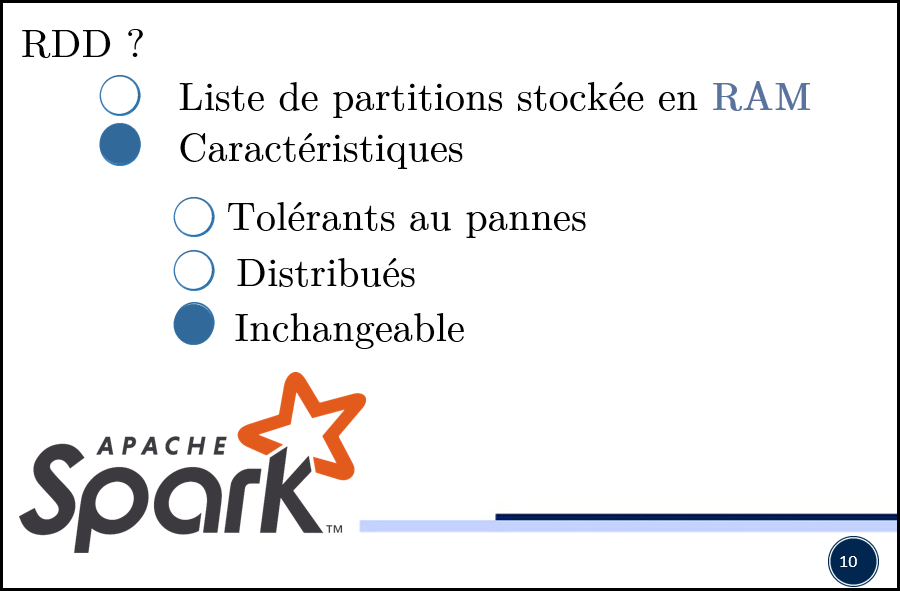
\includegraphics[scale=0.4]{slide8}
\end{center}
\end{figure}


\item N°16 : Élagage de l'arbre de décision.\\
En se basant sur ce que montre le slide, un sous arbre est élagué puis remplacé par un nœud fils, d'autres nœuds (appartenant au sous arbre) seront éventuellement perdus, ce qui affectera la précision de l'arbre de décision, qui a la base, est supposée être optimisée avec l'élagage, ce qui est contradictoire.\\Cette idée est à revoir avec une recherche encore plus approfondie. 

\begin{figure}[!h]
\begin{center}
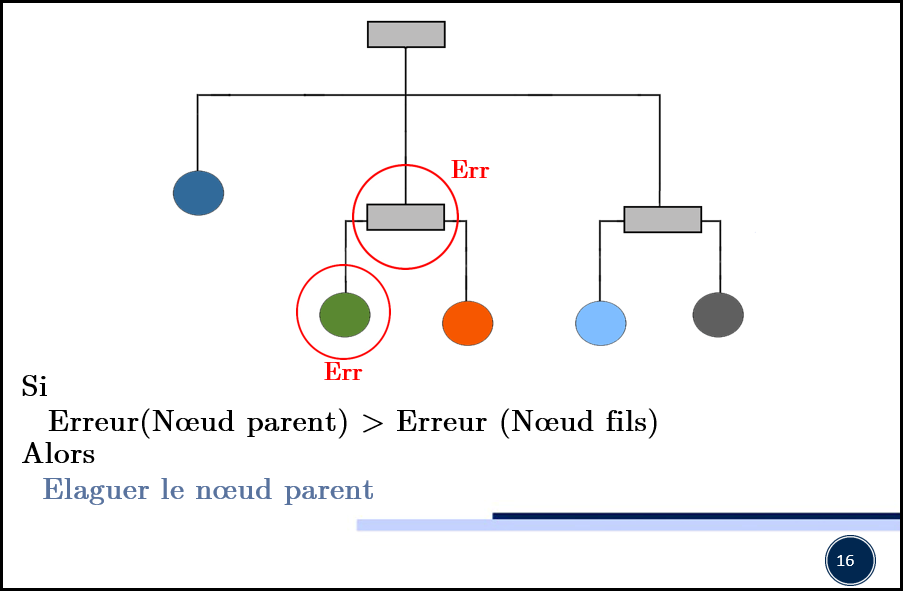
\includegraphics[scale=0.4]{slide16}
\end{center}
\end{figure}



\item N°18 : avantages et inconvénients des arbres de décision.\\
\begin{itemize}
\item Sur quel critère se baser pour estimer qu'un arbre de décision est optimal par rapport à un autre ? (temps?, vitesse?, taille?, autres ?).
\begin{figure}[!h]
\begin{center}
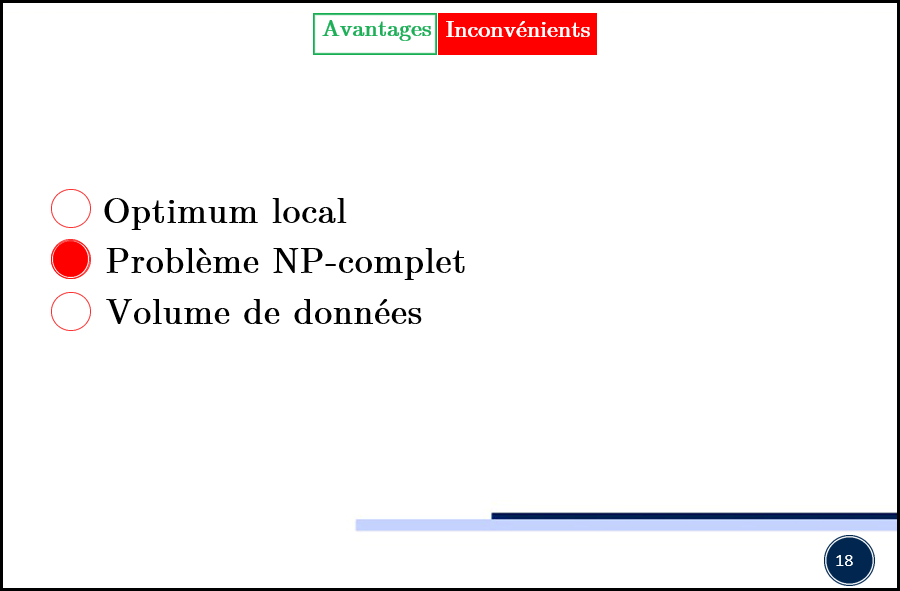
\includegraphics[scale=0.4]{slide18}
\end{center}
\end{figure}


\item Quelle importance doit-on attribuer à chacun de ces critères ? et par rapport a quel contexte ?
\item Ne serait-il pas intéressant de calculer/se rapprocher de l'optimum global, même au détriment de son cout de calcul,  dans des cas ou le besoin d'analyse n'est pas régulier.
\item Les caractéristiques de l'ensemble de données d'apprentissage peuvent-ils avoir un effet sur la qualité de l'arbre de décision produit ? Dans ce cas, quel serait le critère d'un bon jeu de données ? cette idée a elle été abordée sur un des articles des approches proposées ? 
\end{itemize}

\item N° 24, 25 : Les deux approches MReC4.5 et MRID4.\\
Les figures qui ne présente pas de comparaison entre l'approche proposée et celles existantes ne devrait pas être mises.\\ 
\end{enumerate}

\item A préparer pour le mercredi 21\//03\//2018 : 
\begin{enumerate}
\item Pour chacun des critères de division cités :
\begin{itemize}
\item Une définition claire, nette et précise.
\item Déroulement d'un exemple.
\item Expliquer dans quel contexte tel critères est meilleur qu'un autre.
\end{itemize}

\item Définition formel d'un arbre de décision, ainsi que les critères qui permettent d'évaluer, de mesurer et de comparer la qualité des arbres de décision.

\item Explication détaillée de l'idée de la nouvelle approche, et décrire le contexte pour lequel elle pourrait être meilleure que celles déjà existantes.

\end{enumerate}

\end{itemize}

\end{document}
